\fan{TODO: clock()}

Using the recently release Intel SGX SDK, we implmented TC Server as an SGX
application.  The programming model of SGX applications is to seperate out the
security-sensitive part of an application into a trusted partition, while the
remainder of the application is deemed untrusted.  The trusted partition is
later loaded into a SGX enclave and execuate there. 

The idea behind the programming model is that the major body of the application
is just a normal C/C++ application that is execuated as usual. The trusted part
is invoked by the application when the application needs to perform a
security-sensitive task, such as to generate a key pair only unknown to the
trusted part. To call a function in the enclave, the untrusted part first
prepare the arguments and issue a \texttt{EENTER} instruction with the address
of functions being called as arguments.  After the issueing of \texttt{EENTER},
control is transferred to the program insided the enclave until it returns or a
Exit Event happens~\cite{sgxman}. This process is referred to as making
\emph{ecall}s in the SGX documentation.

An SGX enclave is an isolated execution envirtonment where the enclave program
can be loaded and execuated. As a result of being isolated, the flexibility of
enclave programs is trimmed. For example, some instructions, such as IO
instructions and system calls\fan{add more}, are not allowed in the enclave.
Thus an enclave program has no access to the services and resources provided by
operating systems (such as file systems and networking). In order for the enclave
program to make use of OS services, the enclave program first have to exit the 
enclave. The \texttt{EEXIT} takes a function pointer as input and will transfer
control to that address after exiting. Ususally the function being pointed to
is a wrapper function of a system call, where it first make the system call and
gather the result, then it transfer control back to the enclave code so that the
enclave can make use of the data. This process is referred as making \emph{ocall}
in the SGX documentation.

In the context of TC Server, the trusted part implements Figure. \fan{ref to
prog}, which emcompasses a TLS layer, a partical HTTP protocol, a set of
algorithms that can extract information from web pages, and a request handler
that can parse and generate Ethereum transactions and sign it properly with
\skTC.  The untrusted part of TC Server implements Figure \fan{ref to prog},
which roughly emcompasses of two parts: (1) an access point to various OS
services and (2) interfaces with users and Ethereum blockchain. Figure
\ref{fig:tcserver_impl} summarizes these components and their interaction.

\begin{figure}[h]
    \centering
%    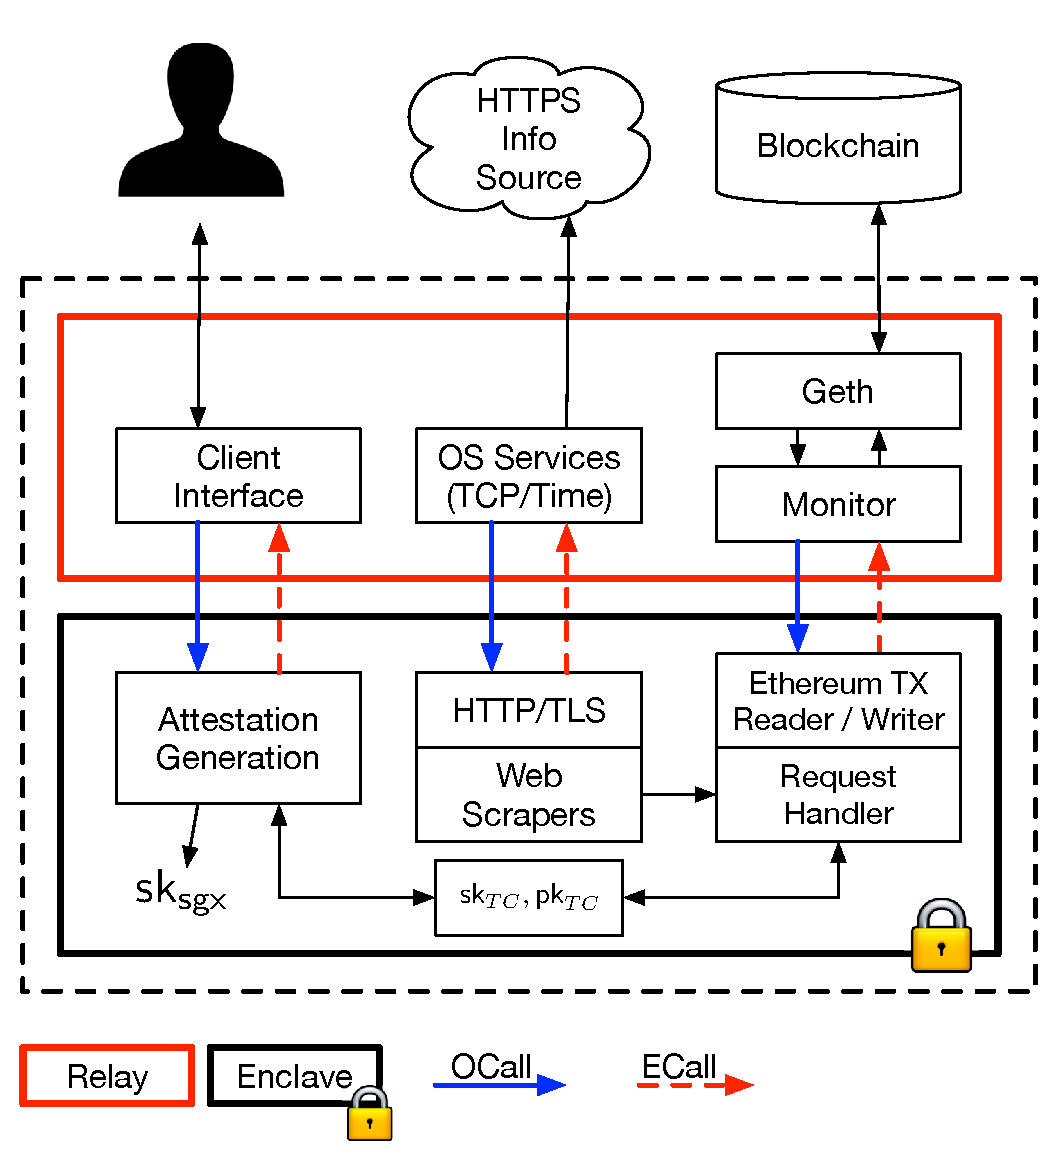
\includegraphics[width=0.4\textwidth]{figures/impl}
    \caption{Detailed Architecture of TC Server}
    \label{fig:tcserver_impl}
\end{figure}

\subsubsection{The \medname}

\paragraph{Attestation Server.} As is described \fan{somewhere}, an user starts
using \tc by requesting an attestation to the \tc server and verifying it.  The
Attestation Server is the interface through which an user can request an
attestation and a unix timestamp signed with \pkTC. An attestation is generated
by sending a report of TC enclave (obtained by \texttt{EGETREPORT}) to the Quoting Enclave(QE). 
QE then verify the report and tag it with an EPID signature signed by \sksgx. 
A SGX attestation can be written as $H(M) || \pkTC || sign(\sksgx, H(M), \pkTC$.
The EPID group signature is used by Intel SGX and users can verify the signature
by access Intel Attestation Server (IAS). 

\paragraph{OS Services.} Enclave relies on \medname to access various services 
provided by OS. For example, TC \medname relies on the TCP service provided by
the OS to transport TLS records. Although OS services are used, they don't need
to be trusted. 

\paragraph{Blockchain Interface.} To interact with the Ethereum blockchain, we
incorporated an offcial Ethereum client (we chose geth in particular) into the
\medname.  Geth client can be configured to set a JSON RPC server through which
the other part of \medname can communicate with the blockchain indirectly. 
For example, to deliver a signed transaction to TC contract, the Monitor can
call \texttt{eth\_sendRawTransaction} RPC call and geth will speak with the blockchain.
By looping an Ethereum client into \medname, we don't have to deal with the Ethereum
specifics.


\subsubsection{The \encname}

\paragraph{HTTPS in the \encname} We ported mbedTLS into SGX style so it can be used within the 
enclave.

\paragraph{Info Extraction} Extracting useful information from a website is implemented
in a ad-hoc manner. For the purpose of demonstration, we implemented three web scrapers
as examples. 

\paragraph{Request Handler} Request handler has two job: 1) to parse the request (decrypt it
if it is encrypted under \pkTC) and dispatch it to the right scraper; 2) to generate a 
Ethereum transaction, sign it with \pkTC and serilize it properly so that it can be
inserted to the blockchain. In essence, we implmented Ethereum ABI and RLP which is use to
serilize arguments and transactions respectively. 
\paragraph{Attestation Generation} The same with Attestation Server.
\paragraph{Key Management} Discuss.
